\documentclass[parskip=full,11pt]{scrartcl}
%\usepackage{pdfpages}
\usepackage[utf8]{inputenc}
\usepackage{amssymb}
\usepackage[T1]{fontenc}
\usepackage[german]{babel}
\usepackage[yyyymmdd]{datetime} 
\usepackage{hyperref}
\usepackage[toc, nonumberlist, automake]{} %added automake option
\usepackage{csquotes}
\usepackage{graphicx}
\usepackage{longtable}
\usepackage{multirow}
\usepackage{pbox}
\usepackage{array}
\newcolumntype{P}[1]{>{\centering\arraybackslash}p{#1}}
\hypersetup{
 		pdftitle={VForWater-Implementierung},
 }
\usepackage{fancyhdr}%<-------------to control headers and footers
\usepackage[a4paper,margin=1in,footskip=.25in]{geometry}
\fancyhf{}
\fancyfoot[C]{\thepage} %<----to get page number below text
\pagestyle{fancy} %<-------the page style itself
 
\title{Qualitätssicherung}
\subtitle{Autorisierungsmanagement für eine virtuelle Forschungsumgebung für Geodaten}
\author{Alex\\Anastasia\\Atanas\\Dannie\\ Houra\\Sonya\\}
\date{11.01.18}
 % define custom lists
\usepackage{enumitem}


\usepackage{linegoal,listings}
\newsavebox{\mylisting}
\makeatletter
\newcommand{\lstInline}[2][,]{%
	\begingroup%
	\lstset{#1}% Set any keys locally
	\begin{lrbox}{\mylisting}\lstinline!#2!\end{lrbox}% Store listing in \mylisting
	\setlength{\@tempdima}{\linegoal}% Space left on line.
	\ifdim\wd\mylisting>\@tempdima\hfill\\\fi% Insert line break
	\lstinline!#2!% Reset listing
	\endgroup%
}
\makeatother
\setlength{\parindent}{0pt}% Just for this example

\lstset{basicstyle=\footnotesize\ttfamily,breaklines=true}
\lstset{framextopmargin=50pt,frame=bottomline,showstringspaces=false,upquote=true}


 
\begin{document}
 
 \begin{titlepage}
 	
 	\begin{center}
 	
\includegraphics[width=0.5\linewidth]{res/KITLogo.png}\\
 	\vspace{2cm}
 	{\scshape\LARGE\bfseries Qualitätssicherung \par}
 	\vspace{0.5cm}
 	{\scshape\Large Praxis der Softwareentwicklung\\}
 	\vspace{1cm}
 	{\scshape\Large Wintersemester 17/18\\}
 	\vspace{2cm}
 	{\huge\bfseries Autorisierungsmanagement für eine virtuelle Forschungsumgebung für Geodaten\par}
 	\vspace{2cm}
 	\vfill
 	{\bfseries {\Large Autoren}:\par}
 	{\Large Bachvarov, Aleksandar }\\
 	{\Large Dimitrov, Atanas }\\
 	{\Large Mortazavi Moshkenan, Houraalsadat }\\
 	{\Large Sakly, Khalil }\\
 	{\Large Slobodyanik, Anastasia }\\
 	{\Large Voneva, Sonya}\\
 	\vfill
 	{\large 14.03.18 \par}
 	\end{center}
 \end{titlepage}
 
 \tableofcontents
 \newpage
 \section{Einleitung}
\begin{center}
\textit{,,Testing shows the presence of bugs, not their absence``}
\end{center}
\begin{flushright}
- Edsger W. Dijkstra\\
\end{flushright}
Das Testen in der Software-Entwicklung ist der Prozess der Untersuchung des Produktes auf Unterschiede zwischen seinem beobachteten Verhalten und dem erwarteten Verhalten des modellierten Systems.
In dem Wasserfall-Vorgehensmodell wird die Testphase direkt vor der Auslieferung des Produktes durchgeführt und als Sicherstellung festgelegter Qualitätsanforderungen betrachtet.\\
Die Testphase ist mit anderen Entwicklungsphasen eng verbunden. Die ersten Tests werden schon in der Implentierungsphase erstellt: Unittests zu jedem View entsprechen dem Komponententest, dessen Ziel ist, Fehler in jedem Teil des Systems aufzufinden. Diese Tests werden im Kapitel \hyperref[komponententest]{\textit{Komponententest}} beschrieben.\\
Das Zusammenspiel einzelner Komponenten wird im Integrationstest geprüft. In dieser Teststufe wird ein Rückblick auf das Artefakt des Entwurfs genommen, um die Integrationsstrategie während dem Test zu berücksichtigen. Tests, die diese Teststufe umschlie{\ss}t, beschreiben wir im Kapitel \hyperref[integrationtest]{\textit{Integrationstest}}.\\
Der abschlie{\ss}ende Teil der Testphase ist der Systemtest, der alle Komponenten zusammen prüft. In unserem Projekt werden dafür manuelle Tests angewendet, die ermöglichen, Benutzerszenarien realitätsnah durchzuarbeiten. Testcases (Testszenarien) in dieser Phase werden anhand funktioneller Anforderungen aus dem Pflichtenheft erstellt und im Kapitel \hyperref[systemtest]{Systemtest} beschrieben.\\
Während der Testphase gefundene und behobene  Defekte werden im Kapitel \hyperref[bugs]{\textit{Aufgetretene Probleme}} erfasst.\\
In der \hyperref[zusammenfassung]{\textit{Zusammenfassung}} werden die Ergebnisse der Testphase betrachtet: Codeüberdeckung vor und nach der Testphase, behobene Fehler und unsere Beurteilung der Lieferfertigkeit des Produktes.
 \newpage
\section{Komponententest} \label{komponententest}
Um die Einzelteile unseres Projekts auf korrektes Verhalten zu überprüfen, wurden sowohl die View-Klassen als auch ihre relevante URLs durch entsprechende Unittest-Klassen getestet. Für jede Test-Klasse werden alle möglichen Fälle durch verschiedene Methoden berücksichtigt.\\
In der vorliegenden Tabelle \ref{kom-tabelle} wird beschrieben, welche Test-Klassen implementiert wurden, was in den jeweiligen Tests geprüft wird und welches Ergebnis erwartet wird.

\begin{longtable}[c]{|p{0.4cm}|P{2.5cm}|p{3.5cm}|p{5cm}|p{3cm}|}
\caption{Komponententest. Jede Test-Klasse (Testcase) testet die entsprechende View-Klasse, indem alle möglichen Fälle durch verschiedene Methoden berücksichtigt werden.}
\label{kom-tabelle}\\
\hline
\textbf{\#} & \centerline{\textbf{Testcase}}&\centerline{\textbf{Methode}}& \centerline{\textbf{Beschreibung}} & \centerline{\textbf{Ergebnis}} \\ \hline
\endfirsthead
%
\endhead
%
\multirow{2}{*}{}1 & \multirow{2}{*}{} TestHomeView & test-not-logged-in & Getestet, ob die ,,Home``-Seite gezeigt wird, wenn man nicht eingeloggt ist. Das wird durch den zurückgegebenen HTTP-Statuscode gemacht.& HTTP Status Code 302: der Benutzer wird zur ,,Login``-Seite weitergeleitet.  \\ \cline{3-5} &   & test-normal & Getestet, ob die ,,Home``-Seite gezeigt wird, wenn man eingeloggt ist.  & HTPP Status Code 200: OK \\ \hline

\multirow{3}{*}{} 2& \multirow{3}{*}{} TestResourceManager&  test-not-logged-in & Getestet, ob die ,,Resource Manager``-Seite gezeigt wird, wenn man nicht eingeloggt ist. & HTTP Status Code 302: der Benutzer wird zur ,,Login``-Seite weitergeleitet \\ \cline{3-5} & & test-logged-in-no-admin & Getestet, ob die ,,Resource Manager``-Seite gezeigt wird, wenn man zwar eingeloggt ist, aber nicht als Admin. & HTTP Status Code 302: der Benutzer wird zur ,,Admin Login``-Seite weitergeleitet \\ \cline{3-5} & & test-normal & Getestet, ob die ,,Resource Manager``-Seite gezeigt wird, wenn man als Admin  eingeloggt ist. & HTPP Status Code 200: OK  \\ \hline

\multirow{3}{*}{} 3& \multirow{3}{*}{} TestUserManager&  test-not-logged-in & Getestet, ob die ,,User Manager``-Seite gezeigt wird, wenn man nicht eingeloggt ist. & HTTP Status Code 302: der Benutzer wird zur ,,Login``-Seite weitergeleitet  \\ \cline{3-5} & & test-logged-in-no-admin & Getestet, ob die ,,User Manager``-Seite gezeigt wird, wenn man zwar eingeloggt ist, aber nicht als Admin. & HTTP Status Code 302: der Benutzer wird zur ,,Admin Login``-Seite weitergeleitet \\ \cline{3-5} & & test-normal & Getestet, ob die ,,User Manager``-Seite gezeigt wird, wenn man als Admin  eingeloggt ist. & HTPP Status Code 200: OK \\ \hline

\multirow{5}{*}{} 4& \multirow{5}{*}{} TestProfileView& test-not-logged-in & Getestet, ob die ,,Profile``-Seite gezeigt wird, wenn man nicht eingeloggt ist.& HTTP Status Code 302: der Benutzer wird zur ,,Login``-Seite weitergeleitet  \\ \cline{3-5} &   & test-normal & Getestet, ob die Profilseite gezeigt wird, wenn man eingeloggt ist.  & HTPP Status Code 200: OK \\ \cline{3-5} 
                  &                   & test-pagination-user & Getestet, ob der Benutzer die zwei Zugriffsrequests sieht, die ihm gesendet wurden. & Anzahl der gezeigten Requests auf der Seite - 2 \\ \cline{3-5} 
                  &                   & test-pagination-admin-page-1 & Getestet, ob der Admin  vier von den fünf Requests, die ihm gesendet wurden,  auf der ersten Seite sieht. & Anzahl der gezeigten Requests auf der ersten Seite - 4 \\ \cline{3-5} 
                  &                   & test-pagination-admin-page-2 & Getestet, ob der Admin  den fünften von den fünf Requests, die ihm gesendet wurden,  auf der zweiten Seite sieht.& Anzahl der gezeigten Requests auf der zweiten Seite - 1 \\  \hline
   
                  
\multirow{3}{*}{} 5& \multirow{3}{*}{} TestMyResourcesView& test-not-logged-in & Getestet, ob die ,,My Resources``-Seite gezeigt wird, wenn man nicht eingeloggt ist.& HTTP Status Code 302: der Benutzer wird zur ,,Login``-Seite weitergeleitet \\ \cline{3-5} &   & test-normal & Getestet, ob die ,,My Resources``-Seite gezeigt wird, wenn man eingeloggt ist.  & HTPP Status Code 200: OK \\ \cline{3-5}& & test-resources-shown & Getestet, ob der Benutzer seine zwei Ressourcen auf der ,,My Resources``-Seite  sieht. &  Anzahl der gezeigten Ressourcen auf der Seite - 2  \\ \hline


\multirow{6}{*}{}6 & \multirow{6}{*}{} TestSendDeletionRequestView& test-not-logged-in & Getestet, ob man einen Löschrequest senden kann, wenn man nicht eingeloggt ist.& HTTP Status Code 302: der Benutzer wird zur ,,Login``-Seite weitergeleitet \\ \cline{3-5} 
                  &                   & test-not-existing-resource &  Getestet, ob man einen Löschrequest für eine Ressource senden kann, wenn die Ressource nicht existiert.  & HTTP Status Code 404: Page not found  \\ \cline{3-5} 
                  &                   & test-not-owner &Getestet, ob ein Benutzer, der die Ressource nicht besitzt, einen Löschrequest senden kann. & HTTP Status Code 403: der Benutzer wird zur ,,Permission Denied``-Seite weitergeleitet    \\ \cline{3-5} 
                  &                   & test-staff-user &Getestet, ob der Admin einen Löschrequest senden kann.  &HTTP Status Code 302: der Admin wird zur ,,My Resources``-Seite weitergeleitet \\ \cline{3-5} 
                  &                   & test-deletion-request-exists  & Getestet, was passiert, wenn man einen Löschrequest sendet und ein Löschrequest für diese Ressource schon existiert.  & HTTP Status Code 302: der Benutzer wird zur ,,My Resources``-Seite weitergeleitet   \\ \cline{3-5} 
                  &                  & test-normal  & Getestet, was im normalen Fall passiert, wenn man einen Löschrequest sendet. & HTTP Status Code 302: der Benutzer wird zur ,,My Resources``-Seite weitergeleitet   \\ \hline
                  
                  
\multirow{6}{*}{}7& \multirow{6}{*}{} TestCancelDeletionRequestView& test-not-logged-in & Getestet, ob man einen Löschrequest stornieren kann, wenn man nicht eingeloggt ist.& HTTP Status Code 302: der Benutzer wird zur ,,Login``-Seite weitergeleitet. \\ \cline{3-5} 
                  &                   & test-not-existing-resource  & Getestet, was passiert, wenn  man versucht einen Löschrequest für eine nicht existierende Ressource zu stornieren.  & HTTP Status Code 404: Page not found  \\ \cline{3-5} 
                  &                   & test-not-owner &Getestet, ob ein Benutzer, der die Ressource nicht besitzt, einen Löschrequest stornieren kann. & HTTP Status Code 403: der Benutzer wird zur ,,Permission Denied``-Seite weitergeleitet   \\ \cline{3-5} 
                  &                   & test-staff-user &Getestet, ob der Admin einen Löschrequest stornieren kann (Admin kann keine Löschrequests senden).  &HTTP Status Code 302: der Benutzer wird zur ,,My Resources``-Seite weitergeleitet.  \\ \cline{3-5} 
                  &                   & test-deletion-request-doesnt-exist  & Getestet, was passiert, wenn man versucht einen nicht existierenden Löschrequest zu stornieren.  &  HTTP Status Code 404: Page not found  \\ \cline{3-5}
                  &                   & test-normal  & Getestet, was im normalen Fall passiert, wenn man einen Löschrequest storniert. & HTTP Status Code 302: der Benutzer wird zur ,,My Resources``-Seite weitergeleitet    \\ \hline
                  
                  
                  
\multirow{4}{*}{}8 & \multirow{4}{*}{} TestApproveAccessRequestView& test-not-logged-in & Getestet, ob man einen Zugriffsrequest genehmigen kann, wenn man nicht eingeloggt ist.& HTTP Status Code 302: der Benutzer wird zur ,,Login``-Seite weitergeleitet   \\ \cline{3-5}  
                  &                   & test-not-existing-request  & Getestet, was passiert, wenn man versucht einen nicht existierenden Zugriffsrequest zu genehmigen.  &  HTTP Status Code 404: Page not found  \\ \cline{3-5}
                  &                   & test-not-owner &Getestet, ob ein Benutzer, der die Ressource nicht besitzt, einen Zugriffsrequest genehmigen kann. & HTTP Status Code 403: der Benutzer wird zur ,,Permission Denied``-Seite weitergeleitet  \\ \cline{3-5}
                  &                   & test-normal  & Getestet, was im normalen Fall passiert, wenn man einen Zugriffsrequest genehmigt. &   HTTP Status Code 302: der Benutzer wird zur ,,Profile``-Seite weitergeleitet \\ \hline
                  
                  
                  
\multirow{4}{*}{} 9& \multirow{4}{*}{} TestDenyAccessRequestView& test-not-logged-in & Getestet, ob man einen Zugriffsrequest ablehnen kann, wenn man nicht eingeloggt ist.& HTTP Status Code 302: der Benutzer wird zur ,,Login``-Seite weitergeleitet  \\ \cline{3-5}  
                  &                   & test-not-existing-request   & Getestet, was passiert, wenn man versucht einen nicht existierenden Zugriffsrequest abzulehnen.  &  HTTP Status Code 404: Page not found    \\ \cline{3-5}
                  &                   & test-not-owner &Getestet, ob ein Benutzer, der die Ressource nicht besitzt, einen Zugriffsrequest ablehnen kann. & HTTP Status Code 403: der Benutzer wird zur ,,Permission Denied``-Seite weitergeleitet  \\ \cline{3-5}
                  &                   & test-normal  & Getestet, was im normalen Fall passiert, wenn man einen Zugriffsrequest ablehnt. &   HTTP Status Code 302: der Benutzer wird zur ,,Profile``-Seite weitergeleitet  \\ \hline
                  
                  
                  
\multirow{6}{*}{} 10& \multirow{6}{*}{} TestSendAccessRequestView& test-not-logged-in & Getestet, ob man einen Zugriffsrequest senden kann, wenn man nicht eingeloggt ist.& HTTP Status Code 302: der Benutzer wird zur ,,Login``-Seite weitergeleitet \\ \cline{3-5} 
                  &                   & test-not-existing-resource &  Getestet, ob man einen Zugriffsrequest für eine Ressource senden kann, wenn die Ressource nicht existiert.  &  HTTP Status Code 404: Page not found   \\ \cline{3-5}
				  &                   & test-reader &Getestet, ob ein Benutzer, der die Ressource schon zugreifen darf, einen Zugriffsrequest senden kann. & HTTP Status Code 302: der Benutzer wird zur ,,Resources Overview``-Seite weitergeleitet  \\ \cline{3-5}
                  &                   & test-staff-user &Getestet, ob der Admin einen Zugriffsrequest senden kann.  &HTTP Status Code 302: der Benutzer wird zur ,,Resources Overview``-Seite weitergeleitet  \\ \cline{3-5}  
                  &                   & test-access-request-exists  & Getestet, was passiert, wenn der Benutzer einen Zugriffsrequest  für eine Ressource sendet, wenn er schon einen gesendet hat. &  HTTP Status Code 302: der Benutzer wird zur ,,Resources Overview``-Seite weitergeleitet    \\ \cline{3-5}
                  &                   &test-normal  & Getestet, was im normalen Fall passiert, wenn man einen Zugriffsrequest sendet.  & HTTP Status Code 302: der Benutzer wird zur ,,Resources Overview``-Seite weitergeleitet    \\ \hline
                  
                  
                  
\multirow{6}{*}{} 11& \multirow{6}{*}{} TestCancelAccessRequestView& test-not-logged-in & Getestet, ob man einen Zugriffsrequest ablehnen kann, wenn man nicht eingeloggt ist.& HTTP Status Code 302: der Benutzer wird zur ,,Login``-Seite weitergeleitet \\ \cline{3-5} 
                 &                   & test-not-existing-resource  & Getestet, was passiert, wenn man versucht einen Zugriffrequest für eine nicht existierende Ressource zu stornieren.  & HTTP Status Code 404: Page not found  \\ \cline{3-5}
                  &                   & test-reader &Getestet, ob ein Benutzer, der die Ressource schon zugreifen darf, einen Zugriffsrequest stornieren kann. & HTTP Status Code 404: Page not found \\ \cline{3-5} 
                  &                   & test-staff-user &Getestet, ob der Admin einen Zugriffsrequest stornieren kann (Der Admin kann keine Zugriffsrequests senden ).  &HTTP Status Code 404: Page not  found \\ \cline{3-5} 
                  &                   & test-deletion-request-doesnt-exist  & Getestet, was passiert, wenn man versucht einen nicht existierenden Zugriffsrequest zu stornieren.  &  HTTP Status Code 404: Page not found   \\ \cline{3-5}

                  &                   &test-normal  & Getestet, was im normalen Fall passiert, wenn man einen Zugriffsrequest storniert.  & HTTP Status Code 302: der Benutzer wird zur ,,Resources Overview``-Seite weitergeleitet    \\ \hline
                  
                  
                  
\multirow{4}{*}{} 12& \multirow{4}{*}{} TestDeleteResourceView& test-not-logged-in & Getestet, ob man eine Ressource löschen kann, wenn man nicht eingeloggt ist.& HTTP Status Code 302: der Benutzer wird zur ,,Login``-Seite weitergeleitet   \\ \cline{3-5} 
                  &                   & test-not-existing-resource  & Getestet, ob man eine nicht existierende Ressource  löschen kann.  &HTTP Status Code 404: Page not found \\ \cline{3-5} 
				  &                   & test-not-staff-user &Getestet, ob der Benutzer, der kein Admin ist, eine Ressource löschen kann.  &HTTP Status Code 302: der Benutzer wird zur ,,My Resources``-Seite weitergeleitet     \\ \cline{3-5} 
                  &                   & test-normal  & Getestet, was im normalen Fall passiert, wenn man eine Ressource löscht.  & HTTP Status Code 302: der Benutzer wird zur ,,My Resources``-Seite weitergeleitet    \\ \hline
                  
                  
\multirow{2}{*}{} 13& \multirow{2}{*}{} TestEditNameView& test-not-logged-in & Getestet, ob man seine Vor- und Nachname ändern kann, wenn man nicht eingeloggt ist.& HTTP Status Code 302: der Benutzer wird zur ,,Login``-Seite weitergeleitet.    \\ \cline{3-5} 
                  &                   & test-normal  & Getestet, was im normalen Fall passiert, wenn man seine Vor- und Nachname ändert.  & HTTP Status Code 302: der Benutzer wird zur ,,Profile``-Seite weitergeleitet.    \\ \hline
                  
                  
\multirow{3}{*}{} 14& \multirow{3}{*}{} TestResourcesOverview& test-not-logged-in & Getestet, ob die ,,Resources Overview``-Seite gezeigt wird, wenn man nicht eingeloggt ist.& HTTP Status Code 302: der Benutzer wird zur ,,Login``-Seite weitergeleitet   \\ \cline{3-5} 
                  &                   &test-normal  & Getestet, ob die ,,Resources Overview``-Seite gezeigt wird, wenn man eingeloggt ist. &  HTPP Status Code 200: OK  \\ \cline{3-5} 
                  &                   &test-pagination-user  & Getestet, ob der Benutzer die vier existierenden Ressourcen auf der Seite sieht. & Anzahl der gezeigten Ressourcen auf der Seite-4   \\ \hline
                  
                  
\multirow{4}{*}{}15 & \multirow{4}{*}{} TestResourcesOverviewSearch& test-not-logged-in & Getestet, ob die ,,Resources Overview Search``-Seite gezeigt wird, wenn man nicht eingeloggt ist. & HTTP Status Code 302: der Benutzer wird zur ,,Login``-Seite weitergeleitet   \\ \cline{3-5} 
                  &                   &test-normal  & Getestet, ob die ,,Resources Overview Search``-Seite gezeigt wird, wenn man eingeloggt ist. &  HTPP Status Code 200: OK     \\ \cline{3-5} 
                  &                   &test-no-query  & Getestet, was passiert, wenn der Benutzer kein Zeichen für die Suchabfrage eingibt. & HTTP Status Code 302: der Benutzer wird zur ,,Resources Overview``-Seite weitergeleitet   \\ \cline{3-5} 
                  &                   & test-valid-query & Getestet, ob der Benutzer alle Ressourcen, deren Namen die eingegebene Zeichen für die Suchabfrage enthalten, sieht.& Anzahl der gezeigten Ressourcen auf der Seite - 1    \\ \hline
                  
                  
\multirow{8}{*}{}16& \multirow{8}{*}{} TestPermissionEditingView& test-not-logged-in &  Getestet, ob man die ,,Edit Permissions``-Seite  einer Ressource sehen kann, wenn man nicht eingeloggt ist.& HTTP Status Code 302: der Benutzer wird zur ,,Login``-Seite weitergeleitet   \\ \cline{3-5}  
                  &                   & test-not-existing-resource-get &  Getestet, ob man die ,,Edit Permissions``-Seite einer Ressource sehen kann, wenn die Ressource nicht existiert.  & HTTP Status Code 404: Page not found  \\ \cline{3-5} 
                  &                   & test-not-existing-resource-post &  Getestet, ob man die Rechte für eine Ressource ändern kann, wenn die Ressource nicht existiert.  &  HTTP Status Code 404: Page not found  \\ \cline{3-5} 
                  &  & test-not-authorized-user &Getestet, ob der Benutzer die ,,Edit Permissions``-Seite einer Ressource sehen kann, wenn er kein Besitzer der Ressource ist.  &  HTTP Status Code 403: der Benutzer wird zur ,,Permission Denied``-Seite weitergeleitet  \\ \cline{3-5} 
                 &   & test-normal-get & Getestet, ob die ,,Edit Permissions``-Seite im normalen Fall gezeigt wird.  & HTPP Status Code 200: OK   \\ \cline{3-5} 
                              &   & test-normal-post & Getestet, ob  man die Rechte für eine Ressource im normalen Fall ändern kann.  & HTTP Status Code 302: der Benutzer wird zur ,,My Resources``-Seite weitergeleitet  \\ \cline{3-5}  
                  &                   & test-pagination-users & Getestet, ob die gezeigten Benutzer (Rechte von Benutzern) auf der Seite 2 sind. & Anzahl der gezeigten Benutzer auf der Seite - 2 \\ \hline
                  
                  
\multirow{8}{*}{} 17& \multirow{8}{*}{} TestPermissionEditingViewSearch& test-not-logged-in &  Getestet, ob man die ,,Edit Permissions Search``-Seite einer Ressource sehen kann, wenn man nicht eingeloggt ist.& HTTP Status Code 302: der Benutzer wird zur ,,Login``-Seite weitergeleitet   \\ \cline{3-5}  
                  &                   & test-not-existing-resource-get &  Getestet, ob man die ,,Edit Permissions Search``-Seite  einer Ressource sehen kann, wenn die Ressource nicht existiert.  & HTTP Status Code 404: Page not found  \\ \cline{3-5} 
                  &                   & test-not-existing-resource-post &  Getestet, ob man die Rechte für eine Ressource ändern kann, wenn die Ressource nicht existiert.  &  HTTP Status Code 302: der Benutzer wird zur ,,Home``-Seite weitergeleitet  \\ \cline{3-5} 
                  &  & test-not-authorized-user &Getestet, ob der Benutzer die ,,Edit Permissions Search``-Seite  einer Ressource sehen kann, wenn er kein Besitzer der Ressource ist.  &  HTTP Status Code 403: der Benutzer wird zur ,,Permission Denied``-Seite weitergeleitet  \\ \cline{3-5} 
                  &                   &test-no-query  &  Getestet, was passiert, wenn der Benutzer kein Zeichen für die Suchabfrage eingibt& HTTP Status Code 302: der Benutzer wird zur ,,My Resources``-Seite weitergeleitet  \\ \cline{3-5}
                 &   & test-normal-get & Getestet, ob die ,,Edit Permissions Search``-Seite im normalen Fall gezeigt wird.  & HTPP Status Code 200: OK   \\ \cline{3-5} 
                                &                   & test-valid-query & Getestet, ob man allen Benutzer (Rechten von Benutzern), deren Namen die eingegebenen Zeichen für die Suchabfrage enthalten, sieht.& Anzahl der gezeigten Benutzer auf der Seite - 1    
       \\ \cline{3-5}                       &   & test-normal-post & Getestet, ob  man die Rechte für eine Ressource im normalen Fall ändern kann.  & HTTP Status Code 302: der Benutzer wird zur ,,My Resources``-Seite weitergeleitet  \\ \hline 

                  
                  
\multirow{3}{*}{} 18& \multirow{7}{*}{} TestAddNewResourceView& test-not-logged-in & Getestet, ob die ,,Add New Resource``-Seite gezeigt wird, wenn man nicht eingeloggt ist.& HTTP Status Code 302: der Benutzer wird zur ,,Login``-Seite weitergeleitet  \\ \cline{3-5} &   & test-normal & Getestet, ob die ,,Add New Resource``-Seite gezeigt wird, wenn man eingeloggt ist.  & HTPP Status Code 200: OK \\ \hline 
                  &                   & test-no-resource-form & Getestet, was passiert, wenn man eine Post-Anfrage ohne Ressourcenlink sendet.   & HTTP Status Code 302: der Benutzer wird zur ,,My Resources``-Seite weitergeleitet   \\ \hline
                  
                  
\multirow{4}{*}{} 19& \multirow{7}{*}{} TestOpenResourceView& test-not-logged-in & Getestet, ob die ,,Open Resource``-Seite gezeigt wird, wenn man nicht eingeloggt ist. & HTTP Status Code 302: der Benutzer wird zur ,,Login``-Seite weitergeleitet  \\ \cline{3-5}
 &                   & test-not-reader & Getestet, ob der Benutzer die ,,Open Resource``-Seite sehen kann, wenn er keine Zugriffsrechte für die Ressource hat.  & HTTP Status Code 403: der Benutzer wird zur ,,Permission Denied``-Seite weitergeleitet   \\ \cline{3-5} 
 &   & test-normal & Getestet, ob die ,,Open Resource``-Seite im normalen Fall gezeigt wird.  & HTPP Status Code 200: OK \\ \hline
                  
                  
\multirow{4}{*}{}20 & \multirow{4}{*}{} TestApproveDeletionRequestView& test-not-logged-in & Getestet, ob man einen Löschrequest genehmigen kann, wenn man nicht eingeloggt ist.& HTTP Status Code 302: der Benutzer wird zur ,,Login``-Seite weitergeleitet   \\ \cline{3-5}  
                  &                   & test-not-existing-request  & Getestet, was passiert, wenn man versucht einen nicht existierenden Löschrequest zu genehmigen.  &  HTTP Status Code 404: Page not found   \\ \cline{3-5}
                  &                   & test-not-admin &Getestet, ob ein Benutzer, der kein Admin ist, einen Löschrequest genehmigen kann. & HTTP Status Code 403: der Benutzer wird zur ,,Permission Denied``-Seite weitergeleitet  \\ \cline{3-5}
                  &                   & test-normal  & Getestet, was im normalen Fall passiert, wenn man einen Löschrequest genehmigt. &   HTTP Status Code 302: der Benutzer wird zur ,,Profile``-Seite weitergeleitet \\ \hline
                  
                  
                  
\multirow{4}{*}{} 21& \multirow{4}{*}{} TestDenyDeletionRequestView& test-not-logged-in & Getestet, ob man einen Löschrequest ablehnen kann, wenn man nicht eingeloggt ist.& HTTP Status Code 302: der Benutzer wird zur ,,Login``-Seite weitergeleitet  \\ \cline{3-5}  
                  &                   & test-not-existing-request   & Getestet, was passiert, wenn man versucht einen nicht existierenden Löschrequest abzulehnen.  &  HTTP Status Code 404: Page not  found   \\ \cline{3-5}
                  &                   & test-not-admin &Getestet, ob ein Benutzer, der kein Admin ist, einen Löschrequest ablehnen kann. & HTTP Status Code 403: der Benutzer wird zur ,,Permission Denied``-Seite weitergeleitet  \\ \cline{3-5}
                  &                   & test-normal  & Getestet, was im normalen Fall passiert, wenn man einen Löschrequest ablehnt. &   HTTP Status Code 302: der Benutzer wird zur ,,Profile``-Seite weitergeleitet  \\ \hline
                  
                  
\end{longtable}
\newpage


\section{Integrationstest} \label{integrationtest}
Integrationstests dienen dazu, das Zusammenspiel aller Komponenten zu überprüfen. Während dieser Phase werden Tests entsprechend der Modularität, welche im Entwurf festgelegt wurde, erstellt. Django-Applications arbeiten nach dem Prinzip ,,Model View Template``, welches die Benutzeraktionen des Templates mit Hilfe der View entnimmt und diese direkt in die Datenbank integriert.\\
Um diese Verbindung zu testen, haben wir automatische Unittests benutzt (Tabelle \ref{it-tabelle} ), die den Datenbankzustand vor und nach der Ausführung der View-Funktionen prüfen.\\

\begin{longtable}[c]{|p{0.4cm}|P{2cm}|p{2cm}|p{5cm}|p{4.5cm}|}
\caption{Integrationstests. Jede Klasse enthält eine Gruppe von Methoden (Testcases), die mit entsprechender Datenart arbeiten. Jede Methode testet einen Vorgang, der in der Beschreibung erläutert wird. Die Ergebnis-Spalte beschreibt das erwartete Verhalten des Systems.}
\label{it-tabelle}\\
\hline
\textbf{\#} & \textbf{Klasse}&\centerline{\textbf{Methode}}& \centerline{\textbf{Beschreibung}} & \centerline{\textbf{Ergebnis}} \\ \hline
\endfirsthead
%
\endhead
%
\multirow{3}{*}{}1 & \multirow{2}{*}{} TestUserdata & 
test-edit-name & Test öffnet die Profilseite des eingeloggten Benutzers und ändert seinen Vor- und Nachnamen. & Neue Vor- und Nachnamen werden in der Datenbank gespeichert.
\\ \cline{3-5} &   & test-my-requests & Test öffnet die Profilseite des eingeloggten Benutzers und fragt die Liste der angezeigten Requests ab. & Die angezeigte Liste entspricht der Liste aller Requests in der Datenbank, die an den Benutzer adressiert sind.
\\ \cline{3-5} &   & test-my-resources & Test öffnet die ,,My Resources``-Seite des eingeloggten Benutzers und fragt die Liste der angezeigten Ressourcen ab. & Die angezeigte Liste entspricht der Liste aller Ressourcen in der Datenbank, für die der Benutzer Besitzerrechte hat. \\ \hline

\multirow{3}{*}{} 2& \multirow{3}{*}{} TestResourcesData&  
test-resources-overview & Test öffnet die ,,Resources Overview``-Seite und fragt die Liste der angezeigten Ressourcen ab. & Die Liste enthält alle Ressourcen, die in der Datenbank gespeichert sind.  
\\ \cline{3-5} & & test-access-permissions & Test öffnet die ,,Resources Overview``-Seite und fragt die Liste der Ressourcen, für die der ,,Access``-Button angezeigt wird, ab. & Die angezeigte Liste entspricht der Liste aller Ressourcen in der Datenbank, für die der Benutzer Zugriffsrechte hat.

\\ \cline{3-5} & & test-resource-permissions & Test öffnet die ,,Edit permissions``-Seite für jede Ressource, die der eingeloggte Benutzer besitzt und fragt die Listen der angezeigten Besitzer- und Zugriffsrechte ab. & Die Listen entsprechen der Listen aller Benutzer, die als Besitzer, bzw. Leser dieser Ressource in der Datenbank gespeichert sind. \\ \hline

\multirow{8}{*}{} 3& \multirow{3}{*}{} TestRequestsData&  
test-create-access-request & Test öffnet die ,,Resources Overview``-Seite und sendet einen Zugriffsrequest für jede Ressource, für die kein ,,Access``-Button angezeigt wird. & Für alle Ressourcen, für die der Benutzer keine Zugriffsrechte hat, werden Zugriffsrequests in der Datenbank gespeichert. 
\\ \cline{3-5} & & test-cancel-access-request & Test öffnet die ,,Resources Overview``-Seite und löscht alle Zugriffsrequests, die angezeigt werden. & In der Datenbank  sind keine Zugriffsrequests von dem Benutzer gespeichert.
\\ \cline{3-5} & & test-create-deletion-request. & Test öffnet die ,,My Resources``-Seite des eingeloggten Benutzers und sendet einen Löschrequest für jede Ressourcen, die angezeigt wird. & In der Datenbank sind Löschrequests für alle Ressourcen, für die der Benutzer Besitzerrechte hat, gespeichert.  
\\ \cline{3-5} & & test-cancesl-deletion-request & Test öffnet die ,,My Resources``-Seite des eingeloggten Benutzers und löscht alle Löschrequests, die angezeigt werden. & In der Datenbank  sind keine Löschrequests von dem Benutzer gespeichert.
\\ \cline{3-5} & & test-accept-access-request & Test öffnet die Profilseite des eingeloggten Benutzers und nimmt alle angezeigten Zugriffsrequests an. & In der Datenbank sind Zugriffsrechte für entsprechende Sender und Ressourcen gespeichert. Bearbeitete Requests werden aus der Datenbank gelöscht.
\\ \cline{3-5} & & test-deny-access-request & Test öffnet die Profilseite des eingeloggten Benutzers und lehnt alle angezeigten Zugriffsrequests ab. & In der Datenbank sind keine Zugriffsrechte für entsprechende Sender und Ressourcen gespeichert. Bearbeitete Requests werden aus der Datenbank gelöscht.
\\ \cline{3-5} & & test-accept-deletion-request & Test öffnet die Profilseite des eingeloggten Admins und nimmt alle angezeigten Löschrequests an. & Bearbeitete Requests und entsprechende Ressourcen werden aus der Datenbank gelöscht.
\\ \cline{3-5} & & test-deny-deletion-request & Test öffnet die Profilseite des eingeloggten Admins und lehnt alle angezeigten Löschrequests ab. & Bearbeitete Requests werden  aus der Datenbank gelöscht und entsprechende Ressourcen bleiben in der Datenbank gespeichert.\\ \hline
                  
                  

\end{longtable}

\newpage
\section{Systemtest} \label{systemtest}
Systemtest im Sinne der Software-Entwicklung ist der abschlie{\ss}ende Test, der vom Entwickler durchgeführt wird. Das Ziel dieses Tests ist das Verhalten des Produkts als Ganzes in einer realen Umgebung (immer noch ohne Kunden) zu beobachten.\\
Im Rahmen unseres Projektes bezeichnen wir manuelle Tests als Systemtests. Sie entsprechen möglichen Szenarien, die durch Interaktion des Benutzers mit dem System entstehen. Als Basis dafür dienen die im Pflichtenheft vordefinierte globale Testfälle. Für die klare Unterscheidung zwischen den verschiedenen Rollen, die man im Portal haben kann, sind die manuelle Tests in drei Gruppen aufgeteilt, die den Benutzer (Tabelle \ref{manTestsBenutzer}), den Besitzer (Tabelle \ref{manTestsBesitzer}) oder den Administrator (Tabelle \ref{manTestsAdmin}) betreffen.\\
Um die Kompatibilität des Produkts mit verschiedenen Umgebungen zu testen, haben wir die Systemtests erfolgreich mit vier modernen Browser (deren Benutzung schon im Pflichtenheft als Kriterium gesetzt wurde) - Chrome, Firefox, Safari und Microsoft Edge auf vier Betriebssystemen - Windows 8, Windows 10, Mac OS 10 und Ubuntu 16 durchgeführt.  

\begin{longtable}[c]{|P{2.5cm}|p{1.0cm}|p{5cm}|p{6.5cm}|}
\caption{Manuelle Tests für den Benutzer: Jeder Testcase (TXXX-Nummer entspricht der Nummer im Pflichtenheft) testet die entsprechende funktionale Anforderung (FA) aus dem Pflichtenheft. Tescases ab T020 implizieren das Einloggen.}
\label{manTestsBenutzer}\\
\hline
\textbf{Testcase}&\textbf{FA}& \textbf{Action} & \textbf{Reaction} \\ \hline
\endfirsthead
%
\endhead
%
\multirow{2}{*}{} T010 : Profilübersicht& \multirow{2}{*}{} F010 & Einloggen &Der ,,Profile``-Button ist angezeigt  \\ \cline{3-4}    &  & Klicke auf den ,,Profile``-Button  &Die Profilseite ist angezeigt: der Benutzername, die Liste der Requests, der ,,My Resources``-Button \\ \cline{3-4}    &  & Ausloggen  &Die Profilseite kann nicht geöffnet werden \\ \hline

\multirow{2}{*}{} T020 : Name editieren & \multirow{2}{*}{} F020 &  Klicke auf den ,,Profile``-Button  &Die Profilseite ist angezeigt: der Benutzername, die Liste der Requests, der ,,My Resources``-Button \\ \cline{3-4}    &  & Klicke auf den Namen & Name- und Vorname-Felder sind angezeigt \\ \cline{3-4}    &  & Schreibe den Namen und Vornamen  &  Die neue Name und Vorname werden in den Felder geschrieben \\ \cline{3-4}    &  & Klicke auf den ,,OK``-Button  & Die neue Name und Vorname werden auf der Profilseite korrekt angezeigt \\ \hline

\multirow{2}{*}{} T030 : Ressourcenzugriff& \multirow{2}{*}{} F030 & Klicke auf den ,,Resources Overview``-Button  & Die Liste der Ressourcen wird angezeigt \\ \cline{3-4}    &  & Klicke auf den ,,Access``-Button  &Das Herunterladen-Fenster wird geöffnet \\ \cline{3-4}    &  & Klicke auf den ,,Speichern``-Button  &Die Ressource wird heruntergeladen \\ \hline

\multirow{2}{*}{} T040 : Ressourcenerstellung & \multirow{2}{*}{} F040 & Klicke auf den ,,Profile``-Button  &Die Profilseite ist angezeigt: Benutzername, Liste der Requests, ,,My Resources``-Button  \\ \cline{3-4}    &  & Klicke auf den ,,My Resources``-Button  &Der ,,Add``-Button (,,+``-Button) und die Liste der Ressourcen sind angezeigt \\ \cline{3-4}    &  & Klicke auf den ,,Add``-Button  &Die Felder: ,,Name``, ,,Type``, ,,Description``, ,,Link`` und der ,,Add``-Button sind angezeigt \\ \cline{3-4}    &  & Fülle die Felder aus, füge einen Link hinzu and klicke auf den ,,Add``-Button  & Zur ,,My Resources``-Seite weitergeleitet, erstellte Ressource ist  in der Liste verfügbar \\ \hline

\multirow{2}{*}{} T050 : Access Request senden& \multirow{2}{*}{} F050 & Klicke auf den ,,Resources Overview``-Button  &Die ,,Resources``-Seite ist angezeigt , einschlie{\ss}lich einer Liste von Ressourcen und eines Suchfeldes \\ \cline{3-4}    &  & Klicke auf den ,,Send Request``-Button  &Der Nachricht-Dialog ist angezeigt , mit optionalem Beschreibungsfeld  , ,,Yes`` und  ,,Close``-Button \\ \cline{3-4}    &  & Klicke auf den ,,Yes``-Button  & Anstatt des ,,Send Request``-Buttons ist der ,,Cancel Request``-Button angezeigt\\ \hline

\multirow{2}{*}{} T060 : Benachrichtigung& \multirow{2}{*}{} F060 & Klicke auf den ,,Resources Overview``-Button  &Die ,,Resources``-Seite ist angezeigt , einschlie{\ss}lich einer Liste von Ressourcen und eines Suchfeldes \\ \cline{3-4}    &  & Klicke auf den ,,Send Request``-Button & Anstatt des ,,Send Request``-Buttons ist der ,,Cancel Request``-Button angezeigt  \\ \cline{3-4}    &  &Die Anfrage Akzeptieren/ablehnen (Aus dem Besitzer-Konto)  & \multirow{2}{*}{} Die Logdatei enthält eine Email und Beschreibung  \\ \cline{3-3}    &  & Öffne die Logdatei  & \\ \cline{3-3}    &  & Suche nach der Email  &  \\ \hline

%\multirow{2}{*}{} T080 : Multiple Request& \multirow{2}{*}{} F080 & Einloggen & ,,Resources Overview``-Button ist angezeigt  \\ \cline{3-4}    &  & Klicke auf ,,Resources Overview``-Button  & ,,Resources``-Seite ist angezeigt , einschließlich einer Liste von Ressourcen und einem Suchfeld \\ \cline{3-4}    &  & Klicke auf ,,Send Request``-Button  & Nachricht Dialog ist angezeigt , mit freiwilligen Beschreibungsfeld  , ,,Yes``- und  ,,Close``-Button \\ \cline{3-4}    &  & Klicke auf ,,Yes``-Button  & ,,Cancel Request``-Button ist nun angezeigt anstatt von ,,Send Request``-Button für alle Ressourcen \\ \cline{3-4}    &  & Klicke auf ,,Send Request``-Button von einer andere Ressource  & Nachricht Dialog ist angezeigt , mit freiwilligen Beschreibungsfeld  , ,,Yes``- und ,,Close``-Button \\ \cline{3-4}    &  & Klicke auf ,,Yes``-Button  & ,,Cancel Request``-Button ist nun angezeigt anstatt von ,,Send Request``-Button für alle Ressourcen \\ \cline{3-4}    &  & Klicke auf ,,Send Request``-Button von einer anderer Ressource  & Nachricht Dialog ist angezeigt , mit freiwilligen beschreibeungsfeld  , ,,Yes``- und ,,Close``-Button \\ \cline{3-4}    &  & Klicke auf ,,Yes``-Button  & ,,Cancel Request``-Button ist nun angezeigt anstatt von ,,Send Request``-Button für alle Ressourcen \\ \cline{3-4}    &  & Klicke auf ,,Send Request``-Button von einer anderer Ressource  & Nachricht Dialog ist angezeigt , mit freiwilligen Beschreibungsfeld  , ,,Yes``- und ,,Close``-Button \\ \cline{3-4}    &  & Öffne die Logdatei  & alle Requests wurden in der Logdatei geschrieben \\ \hline
\end{longtable}


\newpage
\begin{longtable}[c]{|P{2.5cm}|p{1.0cm}|p{5cm}|p{6.5cm}|}
\caption{Manuelle Tests für den Besitzer: Jeder Testcase (TXXX-Nummer entspricht der Nummer im Pflichtenheft) testet die entsprechende funktionale Anforderung (FA) aus dem Pflichtenheft. Alle Testcases implizieren, dass der Benutzer eingeloggt ist.}
\label{manTestsBesitzer}\\
\hline
\textbf{Testcase}&\textbf{FA}& \textbf{Action} & \textbf{Reaction} \\ \hline
\endfirsthead
%
\endhead
%
\multirow{2}{*}{} T220 : Übersicht der Requests& \multirow{2}{*}{} F180 & Klicke auf den ,,Profile``-Button  & Die Liste der erhaltenen Requests wird angezeigt \\ \hline

\multirow{2}{*}{} T230 : Übersicht der Ressourcen& \multirow{2}{*}{} F190 & Klicke auf den ,,Profile``-Button  &Der ,,My Resources``-Button wird angezeigt \\ \cline{3-4}    &  & Klicke auf den ,,My Resources``-Button  &Die Liste der eigenen Ressourcen wird angezeigt  \\ \hline

\multirow{2}{*}{} T240 : Vergabe der Zugriffsrechte& \multirow{2}{*}{} F200 &Auf den ,,Profile``-Button klicken  &Der ,,My Resources``-Button wird angezeigt \\ \cline{3-4}    &  & Auf den ,,My Resources``-Button klicken  &Die Liste der eigenen Ressourcen wird angezeigt, folgende Buttons werden für jede Ressource angezeigt: ,,Access``, ,,Edit Permissions``, ,,Delete`` \\ \cline{3-4}    &  & Klicke auf den ,,Edit Permissions``-Button  &Das ,,Search``-Feld wird angezeigt \\ \cline{3-4}    &  & Schreibe den Benutzernamen und Klicke auf den ,,Search``-Button  &Der Gesuchte Benutzer wird angezeigt \\ \cline{3-4}    &  & Klicke auf den ,,Reader``-Button und ,,Confirm``-Button &Der Benutzer soll als Leser angezeigt werden und der ,,Access``-Button soll jetzt beim Benutzer-Konto angezeigt werden \\ \hline

\multirow{2}{*}{} T250 : Request auf Zugriffsrechte ablehnen& \multirow{2}{*}{} F210 & Klicke auf den ,,Profile``-Button  & Die Liste der erhaltenen Requests wird angezeigt \\ \cline{3-4}    &  & Klicke auf den ,,Deny``-Button  &Die Dialogbox wird angezeigt, sie enthält ein Eingabefeld, einen ,,Yes``- und ,,Close``-Button \\ \cline{3-4}    &  & Klicke auf den ,,Yes``-Button  &Der Request soll nicht mehr angezeigt werden und der Benutzer soll nicht als Reader angezeigt werden  \\ \hline

\multirow{2}{*}{} T260 : Request auf Zugriffsrechte akzeptieren& \multirow{2}{*}{} F210 & Klicke auf den ,,Profile``-Button  & Die Liste der erhaltenen Requests wird angezeigt \\ \cline{3-4}    &  & Klicke auf den ,,Accept``-Button  &Die Dialogbox wird angezeigt, sie enthält ein Eingabefeld, einen ,,Yes`` und ,,Close``-Button \\ \cline{3-4}    &  & Klicke auf den ,,Yes``-Button  &Der Request soll nicht mehr angezeigt werden  \\ \cline{3-4}    &  & Klicke auf den ,,My Resources``-Button, ,,Edit Permission``-Button   &Der Benutzer soll als Leser angezeigt werden \\ \hline

\multirow{2}{*}{} T270 : Vergabe der Besitzerrechte& \multirow{2}{*}{} F220 &Auf den ,,Profile``-Button klicken  & ,,My Resources``-Button wird angezeigt \\ \cline{3-4}    &  & Klicke auf den ,,My Resources``-Button  & Liste der eigenen Ressourcen wird angezeigt,die folgende Buttons werden für jede Ressource angezeigt: ,,Access``, ,,Edit Permissions``, ,,Delete`` \\ \cline{3-4}    &  & Klicke auf den ,,Edit Permissions``-Button  & Das Suchfeld wird angezeigt  \\ \cline{3-4}    &  & Schreibe den Benutzernamen und klicke auf den ,,Search``-Button   & Der gesuchter Benutzer wird angezeigt \\ \cline{3-4}    &  & Klicke auf den ,,Owner``-Button und den ,,Confirm``-Button & Der Benutzer soll als Besitzer angezeigt werden \\ \hline

\multirow{2}{*}{} T280 : Löschrequest senden& \multirow{2}{*}{} F230 &Auf den ,,Profile``-Button klicken  & ,,My Resources``-Button wird angezeigt \\ \cline{3-4}    &  & Klicke auf den ,,My Resources``-Button  & Die Liste der eigenen Ressourcen wird angezeigt, Die folgende Buttons für jede Ressource werden angezeigt: ,,Access``, ,,Edit Permissions``, ,,Delete`` \\ \cline{3-4}    &  & Klicke auf ,,Delete``-Button  & Dialogbox wird angezeigt , sie enthält ein Eingabefeld , einen ,,Yes`` und ,,Close``-Button \\ \cline{3-4}    &  & Klicke auf den ,,Yes``-Button  & Statt von den ,,Delete``-Button wird der ,,Cancel Deletion Request``-Button angezeigt  \\ \hline

\multirow{2}{*}{} T290 : Löschbenachrichtigungen&  \multirow{2}{*}{} F240  &Auf den ,,Profile``-Button klicken  & ,,My Resources``-Button wird angezeigt \\ \cline{3-4}    &  & Klicke auf den ,,My Resources``-Button  & Die Liste der eigenen Ressourcen wird angezeigt, folgende Buttons werden für jede Ressource angezeigt: ,,Access``, ,,Edit Permissions``, ,,Delete`` \\ \cline{3-4}    &  & Klicke auf den ,,Delete``-Button  & Ein Dialogbox wird angezeigt , sie enthält ein Eingabefeld , ein ,,Yes``- und ,,Close``-Button \\ \cline{3-4}    &  & Klicke auf den ,,Yes``-Button  & Der ,,Cancel Deletion Request``-Button wird statt ,,Delete``-Button angezeigt \\ \cline{3-4}    &  & Einloggen als Administrator und klicke auf den ,,Profile``-Button  & Löschrequest wird in der Profilseite angezeigt \\ \cline{3-4}    &  & Klicke auf den ,,Accept``-Button & Ein Dialogbox wird angezeigt , sie enthält ein Schreibfeld , einen ,,Yes``- und ,,Close``-Button \\ \cline{3-4}    &  & Klicke auf den ,,Yes``-Button  & Löschrequest wird in der Profilseite nicht mehr angezeigt \\ \cline{3-4}    &  & Die Logdatei öffnen  & Die Logdatei enthält alle gesendete Emails für alle Besitzern \\ \hline

%\multirow{2}{*}{} T300 : Zugriffsrechte zu mehreren Nutzern vergeben& \multirow{2}{*}{} F250 & Einloggen & ,,Profile``-Button ist angezeigt  \\ \cline{3-4}    &  &Auf ,,Profile``-Button klicken  & ,,My Resources``-Button wird angezeigt \\ \cline{3-4}    &  & Klicke auf ,,My Resources``  & Liste der eigenen Ressourcen wird angezeigt, Folgende Button für jede Ressource werden angezeigt: ,,Access``, ,,Edit Permissions``, ,,Delete`` \\ \cline{3-4}    &  & Klicke auf ,,Edit Permissions``-Button  & Suchen Feld wird angezeigt \\ \cline{3-4}    &  & Schreibe "user" und Klicke auf ,,Search``-Button  & alle Users werden angezeigt \\ \cline{3-4}    &  & Klicke auf ,,Reader``-Button für alle Users und ,,Confirm``-Button  & alle Users sollen als Leser angezeigt werden  \\ \hline

\end{longtable}

\newpage
\begin{longtable}[c]{|P{2.5cm}|p{1.0cm}|p{5cm}|p{6.5cm}|}
	\caption{Manuelle Tests für den Administrator: Jeder Testcase (TXXX-Nummer entspricht der Nummer im Pflichtenheft) testet die entsprechende funktionale Anforderung (FA) aus dem Pflichtenheft. Alle Testcases implizieren, dass der Benutzer mit Administratorrechte eingeloggt ist.}
	\label{manTestsAdmin}\\
	\hline
	\textbf{Testcase}&\textbf{FA}& \textbf{Action} & \textbf{Reaction} \\ \hline
	\endfirsthead
	%
	\endhead
	%
	\multirow{2}{*}{} T110 : Löschrequest ablehnen& \multirow{2}{*}{} F110 & Klicke auf den ,,Profile``-Button  & Eine Liste mit Löschrequests ist zu sehen \\ \cline{3-4}    &  & Auf den ,,Deny``-Button zum gewünschten Request klicken  & Ein Dialogfenster wird angezeigt \\ \cline{3-4}    &  & Das Ablehnen bestätigen  & Die Ressource wird nicht gelöscht und der Request wird aus der Datenbank gelöscht \\ \hline
	
	\multirow{2}{*}{} T120 : Löschrequest genehmigen& \multirow{2}{*}{} F110 & Klicke auf den ,,Profile``-Button  & Eine Liste mit Löschrequests ist zu sehen \\ \cline{3-4}    &  & Auf den ,,Accept``-Button zum gewünschten Request klicken  & Ein Dialogfenster wird angezeigt \\ \cline{3-4}    &  & Die Genehmigung  bestätigen  & Die Ressource und der Request werden aus der Datenbank gelöscht\\ \hline
	
	\multirow{2}{*}{} T130 : Ressource löschen& \multirow{2}{*}{} F120 &Auf den ,,Profile``-Button klicken  & Ein ,,My Resources``-Button ist zu sehen \\ \cline{3-4}    &  & Auf den ,,My Resources``-Button klicken  &Alle Ressourcen, die der Admin besitzt, sind in einer Liste zu sehen \\ \cline{3-4}    &  & Auf den ,,Delete``-Button zur entsprechenden Ressource klicken  &Ein Dialogfenster wird angezeigt \\ \cline{3-4}    &  & Das Löschen bestätigen  &Die Ressource wird von DB gelöscht \\ \hline
	
	\multirow{2}{*}{} T140 : Besitzerrechte geben& \multirow{2}{*}{} F130 & Auf den ,,Manage Resources``-Button klicken  & Eine ,,Admin``-Seite wird geöffnet mit einem Link zur Liste aller Ressourcen \\ \cline{3-4}    &  & Auf den ,,Resources``-Button klicken  & Weiterleitung zur Liste aller Ressourcen \\ \cline{3-4}    &  & Eine Ressource finden und darauf klicken  & Optionen zum Editieren dieser Ressource sowie ihrer Leser und Besitzer werden angezeigt \\ \cline{3-4}    &  & Im ,,Owners``-Feld den Benutzer markieren und auf den ,,Save``-Button klicken  & Der ausgewählte Benutzer ist nun Besitzer dieser Ressource \\ \hline
	
	\multirow{2}{*}{} T150 : Besitzerrechte entziehen& \multirow{2}{*}{} F130 & Auf den ,,Manage Resources``-Button klicken  & Eine ,,Admin``-Seite wird geöffnet mit einem Link zur Liste aller Ressourcen \\ \cline{3-4}    &  & Auf den ,,Resources``-Button klicken  & Weiterleitung zur Liste aller Ressourcen \\ \cline{3-4}    &  & Eine Ressource finden und darauf klicken  & Die Optionen zum Editieren dieser Ressource sowie ihrer Leser und Besitzer werden angezeigt\\ \cline{3-4}    &  & Im ,,Owners``-Feld den Benutzer demarkieren und auf den ,,Save``-Button klicken  & Der ausgewählte Benutzer ist nicht mehr Besitzer dieser Ressource \\ \hline
	
	\multirow{2}{*}{} T160 : Zugriffsrechte geben& \multirow{2}{*}{} F130 & Auf den ,,Manage Resources``-Button klicken  & Eine ,,Admin``-Seite wird geöffnet mit einen Link zur Liste aller Ressourcen \\ \cline{3-4}    &  & Auf den ,,Resources``-Button klicken  & Weiterleitung zur Liste aller Ressourcen \\ \cline{3-4}    &  & Eine Ressource finden und darauf klicken  & Die Optionen zum Editieren dieser Ressource sowie ihrer Leser und Besitzer werden angezeigt \\ \cline{3-4}    &  & Im ,,Readers``-Feld den Benutzer markieren und auf den ,,Save``-Button klicken  & Der ausgewählte Benutzer ist nun Leser dieser Ressource \\ \hline
	
	\multirow{2}{*}{} T170 : Zugriffsrechte entziehen& \multirow{2}{*}{} F130 & Auf den ,,Manage Resources``-Button klicken  & Eine ,,Admin``-Seite wird geöffnet mit einen Link zur Liste aller Ressourcen \\ \cline{3-4}    &  & Auf den ,,Resources``-Button klicken  & Weiterleitung zur Liste aller Ressourcen \\ \cline{3-4}    &  & Eine Ressource finden und darauf klicken  & Die Optionen zum Editieren dieser Ressource sowie ihrer Leser und Besitzer werden angezeigt \\ \cline{3-4}    &  & Im ,,Readers``-Feld den Benutzer demarkieren und auf den ,,Save``-Button klicken  & Der ausgewählte Benutzer ist nicht mehr Leser dieser Ressource \\ \hline
	
	\multirow{2}{*}{} T180 : Konto und Daten eines Benutzers löschen& \multirow{2}{*}{} F140 & Auf den ,,Manage Users``-Button klicken  & Die ,,Admin``-Seite wird geöffnet mit einen Link zur Liste aller Users \\ \cline{3-4}    &  & Auf den ,,Users``-Button klicken  & Eine Liste mit allen Benutzern und ein Suchfeld werden angezeigt \\ \cline{3-4}    &  & Einen Benutzer finden und auf seinen Benutzernamen klicken  & Die Optionen zum Editieren der Daten dieses Benutzers \\ \cline{3-4}    &  & Auf den ,,Delete``-Button klicken  & Ein Bestätigungsdialog wird geöffnet \\ \cline{3-4}    &  & Das Löschen bestätigen  & Der ausgewählte Benutzer (und seine Requests) werden gelöscht \\ \hline
	
	\multirow{2}{*}{} T210 : Nach einem Benutzer suchen und ihn blockieren& \multirow{2}{*}{} F160, F170 & Auf den ,,Manage Users``-Button klicken  & Eine ,,Admin``-Seite wird geöffnet mit einen Link zur Liste aller Users \\ \cline{3-4}    &  & Auf den ,,Users``-Button (unter Authentication and Authorization) klicken  & Eine Liste mit allen Benutzern und ein Suchfeld werden angezeigt \\ \cline{3-4}    &  & Einen Benutzer finden und auf seinen Benutzernamen klicken  & Die Optionen zum Editieren der Daten dieses Benutzers \\ \cline{3-4}    &  & Den Haken von ,,Active`` entfernen und auf den ,,Save`` Button klicken  & Der ausgewählte Benutzer kann das Portal (temporär) nicht benutzen  \\ \hline
\end{longtable}
\newpage
\section{Aufgetretene Probleme} \label{bugs}
Während der Testphase sind einige Fehler aufgetreten. Diese Fehler wurden von uns in einem Bugtracker (basiert auf Trello) erfasst und bearbeitet. Jeder Fall wurde nach der Art des Fehlers klassifiziert:

\renewcommand{\labelitemii}{$\bullet$}
\begin{itemize}
\item[] \textbf{Applikationslogik}\\\\
Folgende Fehler waren für Konsistenz des Systems kritisch und mussten umgehend behoben werden.
	\begin{itemize}
		\item \textit{Problem:}\\ Eine eingegebene Nachricht des Administrators beim Ablehnen eines Löschrequests wird in der Email-Benachrichtigung  nicht angezeigt.\\
			\textit{Lösung:}\\ Erweiterung des Email-Templates
		\item \textit{Problem:} \\Auf der Seite ,,Resources overview`` wird kein ,,Access``-Button für eine Ressource  angezeigt, wenn der Benutzer die Besitzerrechte für diese Ressource von einem Administrator bekommen hat.\\
		\textit{Lösung:} \\Wird der Benutzer in ,,owners``-Liste der Ressource hinzugefügt, so wird er auch zur ,,readers`` eingebunden.
		
		\item \textit{Problem:}\\
		Löschrequests von einem Benutzer werden nicht gelöscht, wenn seine Besitzerrechte entzogen werden.\\
		\textit{Lösung:}\\
		Werden Besitzerrechte entzogen, so werden auch alle existierende Löschrequests mit entsprechenden Sender und Ressource als Attribute gelöscht.
		\item \textit{Problem:}\\
		Der Zugriffsrequest von einem Benutzer wird nicht gelöscht, wenn dem die Zugriffsrechte manuell hinzugefügt werden.\\
		\textit{Lösung:}\\
		Werden Zugriffsrechte manuell hinzugefügt, so werden auch alle existierende Zugriffsrequests mit entsprechenden Sender und Ressource als Attribute gelöscht.
	\end{itemize}

\item[]\textbf{Sicherheit}\\\\
Folgende Fehler haben auf die Schwachstellen des Systems und der Datensicherheit verwiesen und mussten umgehend behoben werden.
	\begin{itemize}
		\item \textit{Problem:}\\
		Ein Benutzer kann eine Ressource zugreifen, nach dem seine Zugriffsrechte gelöscht wurden, so lange die Seite mit dem ,,Access``-Button nicht aktualisiert wird.\\
			\textit{Lösung:}\\ Zweistufige Überprüfung der Rechte.		
		\item \textit{Problem:}\\
		Einige Daten (Benutzername, Metadaten) können nach dem Ausloggen des Benutzers aus dem Browser-Cache abgerufen werden.\\
			\textit{Lösung:}\\ Cache der Seiten nicht erlauben.
	\end{itemize}

\item[] \textbf{Fehlerbenachrichtigung}\\\\
In folgenden Fällen hat angemessenes Feedback des Systems gefehlt. Diese Defekte wurden durch Weiterleitung zu entsprechenden Fehlerseiten behoben.
	\begin{itemize}
		\item Bearbeitung eines Requests, der vom Sender gelöscht wurde. 
		\item Bearbeitung eines Requests, falls die entsprechende Ressource gelöscht wurde.
	\end{itemize}
			
\item[] \textbf{Benutzerfreundlichkeit}\\\\
Folgende Defekte hatten zwar keinen Einfluss auf die Konsistenz des Systems, konnten aber einige Schwierigkeiten für Benutzer darstellen.
	\begin{itemize}
		\item \textit{Problem:}\\ Die Benutzersuche auf der ,,Edit permissions``-Seite ausschlie{\ss}lich mit dem Benutzernamen möglich.\\
			\textit{Lösung:} \\Erweiterung der Suchmethode: die Suche mit Email, Vor- und Nachnamen hinzugefügt.
		\item \textit{Problem:}\\ Ein Administrator kann Rechte für seine eigenen Ressourcen nur durch ,,Manage resources''-View ändern.\\
			\textit{Lösung:} \\Ein Administrator kann ,,Edit permissions``-View auf der Seite ,,My resources`` öffnen.
		\item \textit{Problem:}\\ Aufwendige Änderung der Rechte durch Seitenunterteilung.\\
			\textit{Lösung:} \\Im ,,Edit permissions``-View werden zehn statt vier Benutzer pro Seite angezeigt.
	\end{itemize}
	
\item[] \textbf{Benutzeroberfläche}\\\\
Folgende Defekte wurden in der Benutzeroberfläche gefunden. Behebung dieser Defekte hat die Benutzerfreundlichkeit des Produktes verbessert.
	\begin{itemize}
		\item \textit{Problem:}\\ Unbegrenzte Eingabe in einigen Textfelder möglich.\\
			\textit{Lösung:}\\ Änderung des Feldtyps und eingabe maximaler Länge.
		\item \textit{Problem:}\\ ,,Access``-Button nicht auf der ganzen Fläche anklickbar.\\
			\textit{Lösung:}\\ Löschung des Links vom Button-Überschrift.
		\item \textit{Problem:}\\ Der Name der Ressource wird auf der ,,Edit permissions``-Seite nicht angezeigt.\\
			\textit{Lösung:}\\ Erweiterung des Templates.
		\item \textit{Problem:}\\ Der Name des Benutzers kann durch Eingabe des Leerzeichen als neuen Wert gelöscht werden.\\
			\textit{Lösung:}\\ Begrenzung der erlaubten Textfeld-Mustern.
	\end{itemize}
	
\end{itemize}   

\newpage
\section{Zusammenfassung} \label{zusammenfassung}
Während der Testphase unseres Projektes wurden unterschiedliche Testverfahren angewendet. Mit der Django-Funktionalitäten wurden automatische Tests erstellt und ausgeführt: 91 Unittests und 14 Integrationstests verschaffen eine Codeüberdeckung über 90\% (Abbildung \ref{coverage}). \\

 \begin{figure}[ht!]
 	\centering
 	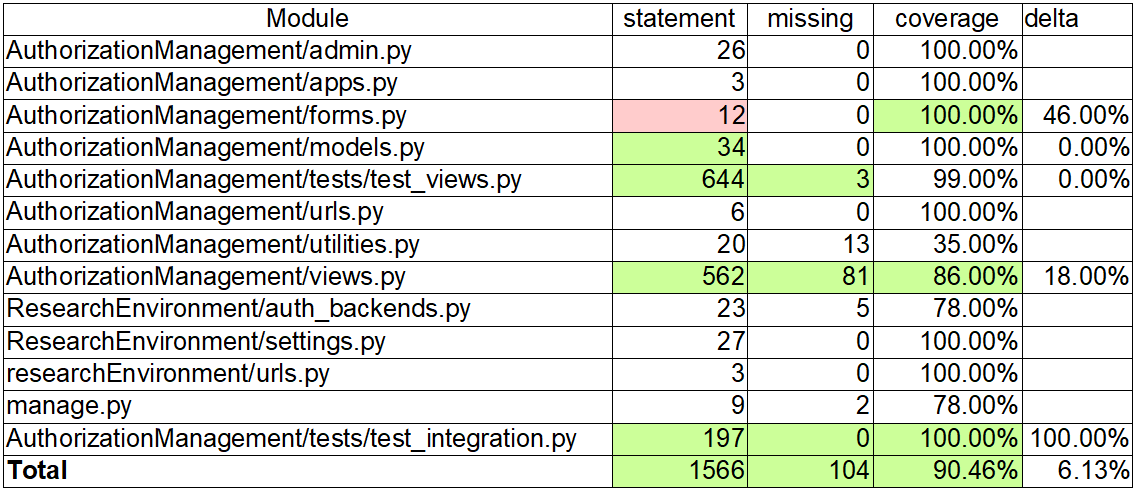
\includegraphics[width=1\textwidth]{res/coverage_after.PNG}
 	\caption{Codeüberdeckung nach der Testphase. Grün sind Werte, die sich während der Testphase verbessert haben, markiert. Rot sind reduzierte Werte markiert. In der Spalte \textbf{delta} wird positive Differenz zwischen Überdeckung vor und nach der Testphase gezeigt.}
\label{coverage}
 \end{figure}
 Als Systemtest wurden 25 manuellen Test entsprechend dem Pflichtenheft definiert und in ausführlichen Szenarien mit mehreren Benutzer in realer Umgebung ausgeführt.\\
Während dem Testen wurden 16 Probleme aufgefunden und behoben. Somit ist die Testphase abgeschlossen und das Produkt ist bereit für Einsatz und Wartung. 
\end{document}
\grid
